%% February 2017, 

\documentclass[12pt, notes=show]{beamer}
\usetheme[width=0cm]{Goettingen}
\usecolortheme{rose}
\useoutertheme{default}
\setbeamerfont{caption}{size=\scriptsize}
\setbeamertemplate{navigation symbols}{}

\addtobeamertemplate{navigation symbols}{}{%
	\usebeamerfont{footline}%
	\usebeamercolor[fg]{footline}%
	\hspace{1em}%
	$\dfrac{\insertframenumber}{\inserttotalframenumber}$
}

\usepackage{hyperref}
\usepackage{fontspec} 
\setsansfont{Futura LT}


\usepackage{arydshln}
\usepackage{amsmath}

\usepackage{mathptmx}
\usepackage{latexsym}
\usepackage{mathtools}
\usepackage{multirow}
\usepackage{caption}
\usepackage{array}
\usepackage{listings}



\title{
	Cultural Evolution \& Economy\\
	Historical Evidences
}

\institute{Septembre 2017}

\author{Simon Carrignon}

\date{
	\scriptsize
	\begin{columns}
		\begin{column}{.3\textwidth}
			\begin{center}
				Barcelona Supercomputing Center	\\
				
\includegraphics[height=1cm]{../../logos/bscLogo.jpg} \hspace{2cm}
			\end{center}
		\end{column}
		\begin{column}{.3\textwidth}
			\begin{center}
				Univ. Pompeu Fabra Complex System Lab.\\
				
\includegraphics[height=1cm]{../../logos/upf_word_imp.jpg} %declare logo image with an alias here 
			\end{center}
		\end{column}
	\end{columns}

}
\begin{document}
\begin{frame}
	\maketitle

\end{frame}

\section{Introduction}

\begin{frame}{Cultural Evolution}
    Social Traits:
    \begin{center}
	\begin{table}
	    \center
	    \begin{tabular}{ccc}
		\uncover<2->{\includegraphics[height=3cm]{images/m80}} &
		\uncover<3->{\includegraphics[height=3cm]{images/m90}} &
		\uncover<4->{\includegraphics[height=3cm]{images/m10}} \\
		\uncover<2->{80's} & \uncover<3->{90's} & \uncover<4->{now}
	    \end{tabular}
	\end{table}
    \end{center}
    \uncover<5->{How they Evolve?}\uncover<6>{ Cultural Evolution }
\end{frame}


\begin{frame}{Cultural Evolution}
    \begin{itemize}
	\item<5->{ culturally transmitted, socially learnt}
	\item<6->{ similar patterns}
    \end{itemize}
	\begin{center}
		\uncover<4->{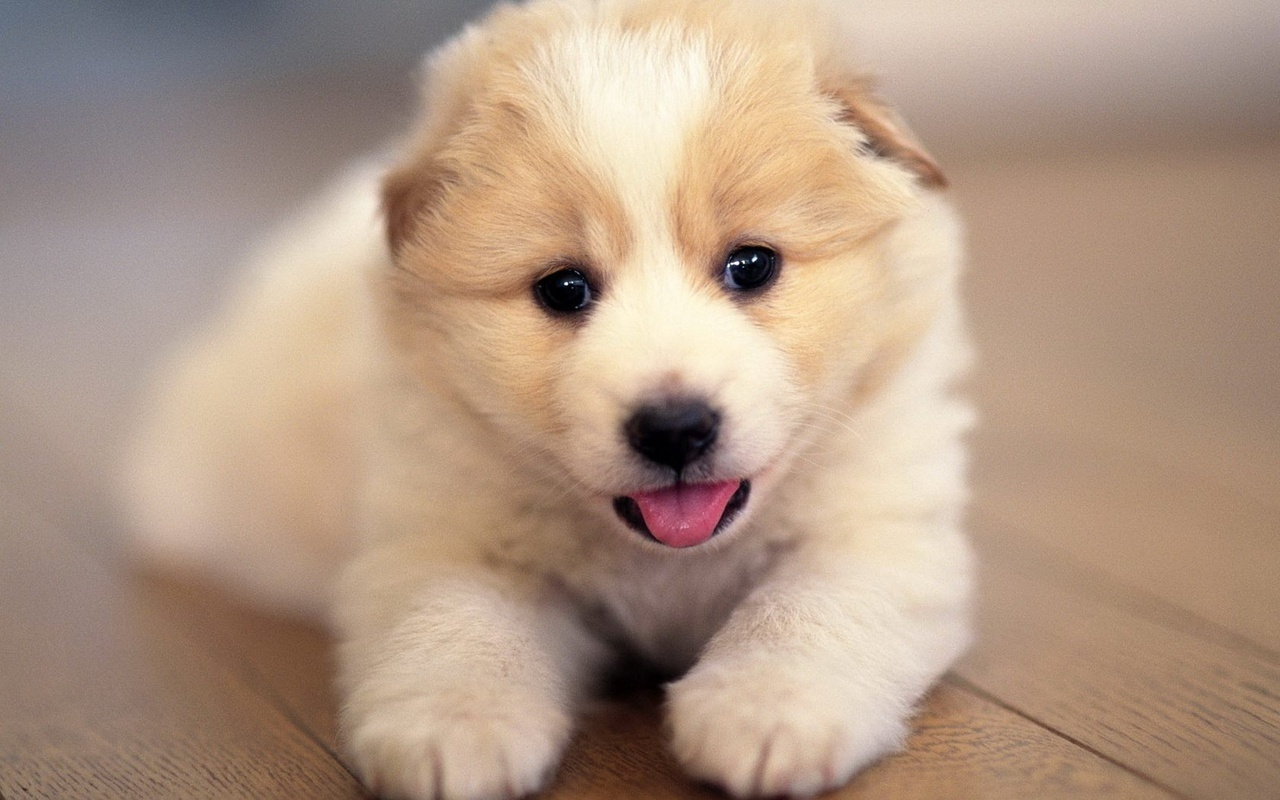
\includegraphics[width=3cm]{images/cutdog}}\\
		\vspace{.5cm}
		\uncover<2->{\includegraphics[width=2.5cm]{images/cutbaby}}
	    \hspace{1cm}
	    \uncover<3->{ \includegraphics[width=2cm]{images/pottery}}
	\end{center}
    \uncover<7>{$\rightarrow$ What mechanism drive the evolution of such traits?\\
    \invisible<1->{$\rightarrow$ What mechanism }generate such pattern?}
\end{frame}

\begin{frame}{What Generate Those Cultural changes?}
	Simple mechanisms (Bentley et al, 2004):
	\begin{itemize}
		\item<2->Random Copy 
		\item<3-> Frequency biased (conformist/anti-conformist\dots)
		\item<4->\dots	
	\end{itemize}
	\uncover<2>{\begin{figure}
		\begin{columns}
			\begin{column}{.8\textwidth}
				\centering
				\includegraphics[width=.6\textwidth]{images/powerlawrepartition.jpg}
			\end{column}
			\begin{column}{.3\textwidth}
				\tiny
				Square: male names\\
				Circle: female names\\
				Dotted and plain lines: model result with different copy probabilities.\\
			From Bentley et al,~2004.
			\end{column}
		\end{columns}
	    \end{figure}}
\end{frame}

\section{Economic Traits}


\begin{frame}
	\begin{center}
	    What if such mechanisms act on traits linked to economics?
	\end{center}
\end{frame}

\begin{frame}{A social traits an economic weight}
	\begin{center}
	    \only<1>{\includegraphics[width=.8\textwidth]{images/boubou1.png}}
	    \only<2>{\includegraphics[width=.8\textwidth]{images/boubou2.png}}
	    \only<3>{\includegraphics[width=.8\textwidth]{images/boubou3.png}}
	\end{center}
\end{frame}

\begin{frame}{Co-evolution of Economy and Culture}

%How Simple Cultural Dynamics influence Economy That in turn will influence cultural dynamics.
    \vspace{2cm}
    \begin{center}
	\begin{overlayarea}{\textwidth}{\textheight}
	    \only<1>{\includegraphics[width=\textwidth]{images/map1.png}}
	    \only<2>{\includegraphics[width=\textwidth]{images/map2.png}}
	    \only<3>{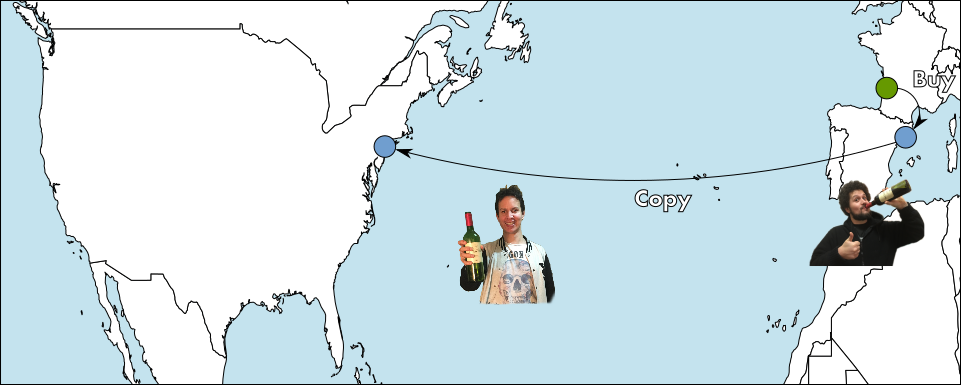
\includegraphics[width=\textwidth]{images/map3.png}}
	    \only<4>{\includegraphics[width=\textwidth]{images/map4.png}}
	    \only<5>{\includegraphics[width=\textwidth]{images/map5.png}}
	    \only<6>{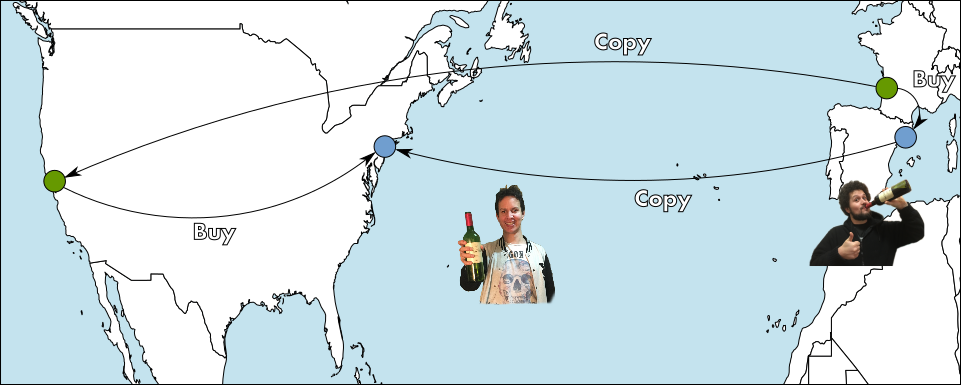
\includegraphics[width=\textwidth]{images/map6.png}}
	    \only<7>{\includegraphics[width=\textwidth]{images/map7.png}}
	    \only<8>{\includegraphics[width=\textwidth]{images/map8.png}}
	    \only<9>{\includegraphics[width=\textwidth]{images/map9.png}}
	    %\only<10>{\includegraphics[width=\textwidth]{images/map10.png}}
	    %\only<11>{\includegraphics[width=\textwidth]{images/graph1.png}}
	    %\only<12>{\includegraphics[width=\textwidth]{images/graph2.png}}
	    %\only<13>{\includegraphics[width=\textwidth]{images/graph3.png}}
	\end{overlayarea}

    \end{center}
\end{frame}



\begin{frame}{Cryptocurrencies}
    \begin{figure}
	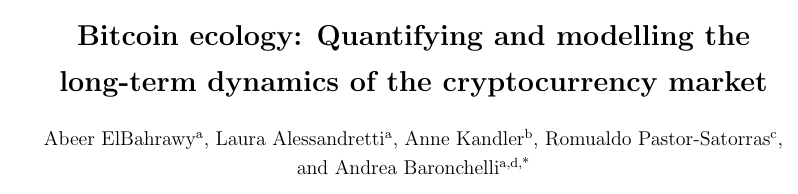
\includegraphics[width=\textwidth]{images/btccultevoabstract.png}\\
    \end{figure}

    A way to exchange values and goods, people will, should, choose the ``best''?
\end{frame}

\begin{frame}{Yet another neutral model}
    Lot's of properties follow a notral model
    \begin{figure}
	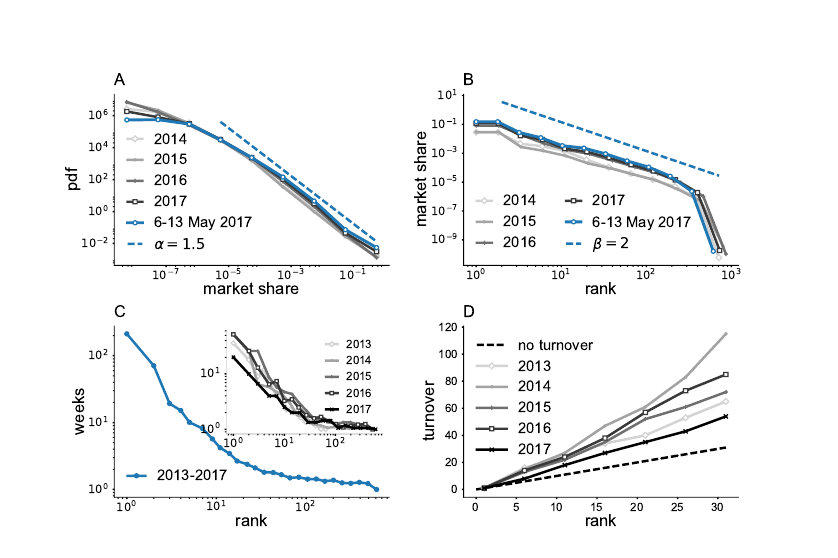
\includegraphics[width=.6\textwidth]{images/btcpic.png}
    \end{figure}

    They conclue:
    \begin{figure}
	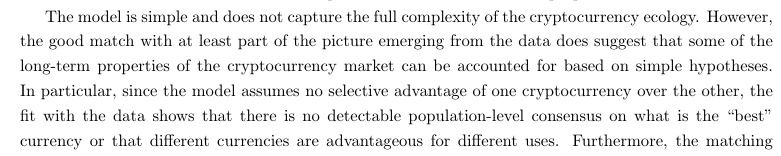
\includegraphics[width=\textwidth]{images/btcNoBest.png}
    \end{figure}
\end{frame}

\section{ABM Framework}


\begin{frame}{General Framework}
    
    \begin{center}
	\includegraphics[width=.8\textwidth]{images/cooev.png}	
    \end{center}
\end{frame}

\begin{frame}{Computer Model}
    \vfill
    Agent Based Model
    \begin{center}
	\includegraphics[width=.5\textwidth]{images/cooev.png}	
    \end{center}
    \vfill
	\begin{itemize}
	\item Different Cultural Mechanisms
    \vfill
	\item Different Trade Assumption
    \vfill
	\item Historical and Archaeological Evidences 
    \vfill
	\item Network Constraints
    \vfill
	\item \dots
    \vfill
	\end{itemize}
\end{frame}
	


\begin{frame}{Results: Economic Dynamics}
	\begin{figure}
	    \caption{Example for 3 goods and 500 agents}
	    \begin{columns}
		\column{.5\textwidth}
		\includegraphics[height=\textwidth]{images/ClearingPriceDistanceEvolutionForTrade-G3N500.pdf}\\
	    \end{columns}
		@~Equilibrium: personal values  $\rightarrow$ optimal (shared) values.
	\end{figure}
	
\end{frame}


\begin{frame}{Economic}
    Model used by economists (Gintes and mandel, Chen et al) to test certains economic assumption
    
\end{frame}

\begin{frame}
    Compare it to Historical Case studies
    
\end{frame}

\begin{frame}{Historical Case Study}
    \footnotesize
    \vspace{.5cm}
Change in distribution of Tableware in the East Roman Empire, -25BC 150AC:
    \begin{itemize}
	\item 5 types of wares 
	\item Distribution among 222 sites
	\item 5121 ware dataset
 \end{itemize}

 \begin{figure}
     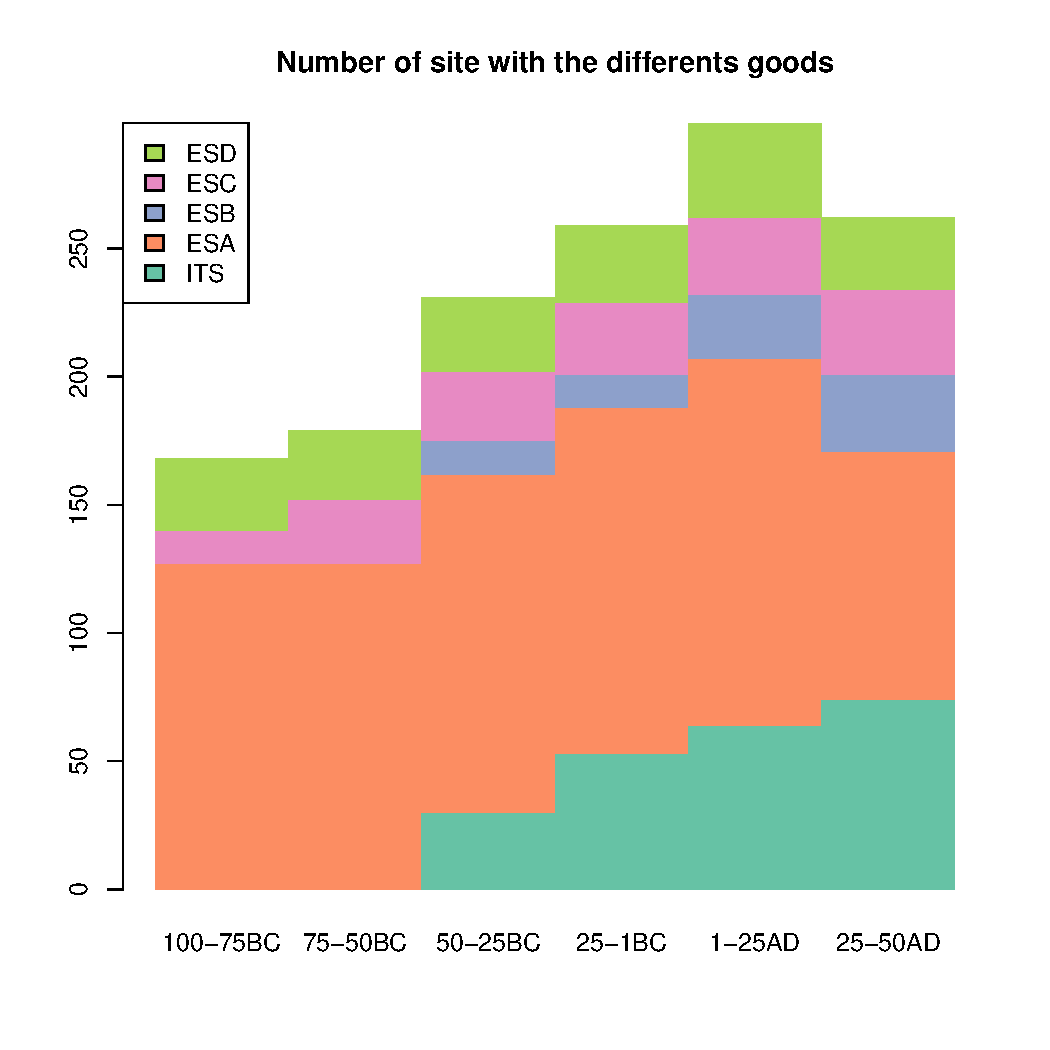
\includegraphics[width=.45\textwidth]{../images/hmNbSiteWGoodData.pdf}
     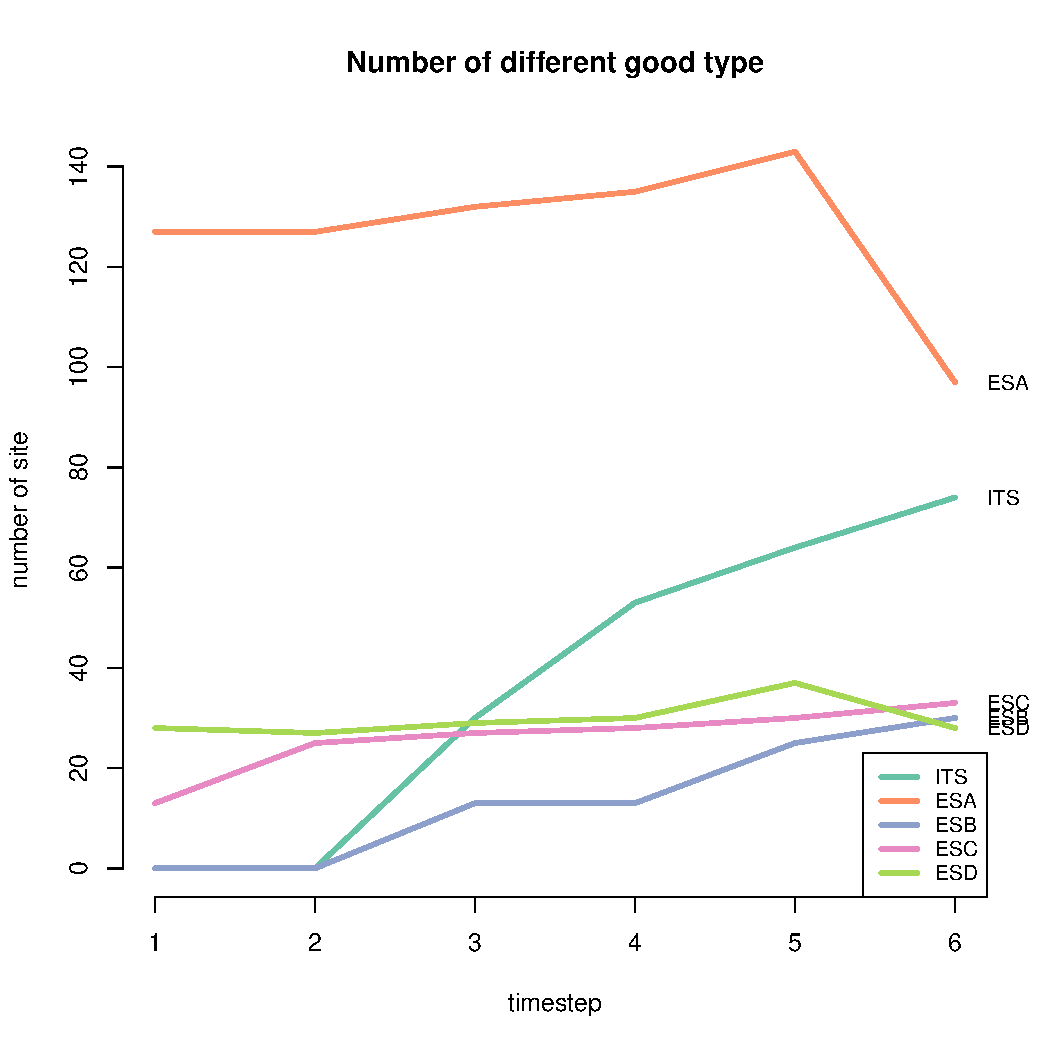
\includegraphics[width=.45\textwidth]{../images/plotNbSiteWGoodData.pdf}
     
 \end{figure}
\end{frame}

\begin{frame}{Specification of the model}
    Simulations with ``real'' parameters:
    \begin{itemize}
	\item 1000 agents
	\item 5 goods (+money) to appear 
	\item 200 ``cultural'' steps 
	\item 3000 ``trade'' steps ($15\times200$)
	\item every 40 cultural steps (ie $600$ trade step) a new good appears.
	\item $\approx 35min$
    \end{itemize}
\end{frame}

\begin{frame}{Experimental framework}
    \begin{itemize}
	\item Test change in $\mu$ the innovation rate (``I randomly change a price'')
	\item Test change in $\lambda$, factor to increase the proba. to copy someone better than me
	\item ( also $\mu$ amplitude, \emph{ie} amplitute of price change when I decide to do so, not shown here)
    \end{itemize}
\end{frame}
\begin{frame}{Parameter tested}
    \begin{itemize}
	\item $\lambda \in \{0.0001,0.001,0.01,0.1,1,10\}$
	\item $\mu \in \{0.001,0.01,0.1,1\}$
	\item  $ 6 \times 4 = 24$ setup, 50s simulation each
    \end{itemize}
\end{frame}

\begin{frame}{Result}
    Check how changes modify general properties:
    \begin{table}
	\centering
	\begin{tabular}{c m{2.5cm}c m{2.5cm}}
	    \multicolumn{2}{c}{\vspace{-1cm}\tiny Quantities at the end} &\multicolumn{2}{c}{\tiny prices at the end}\\
	    \multirow{1}{2.5cm}{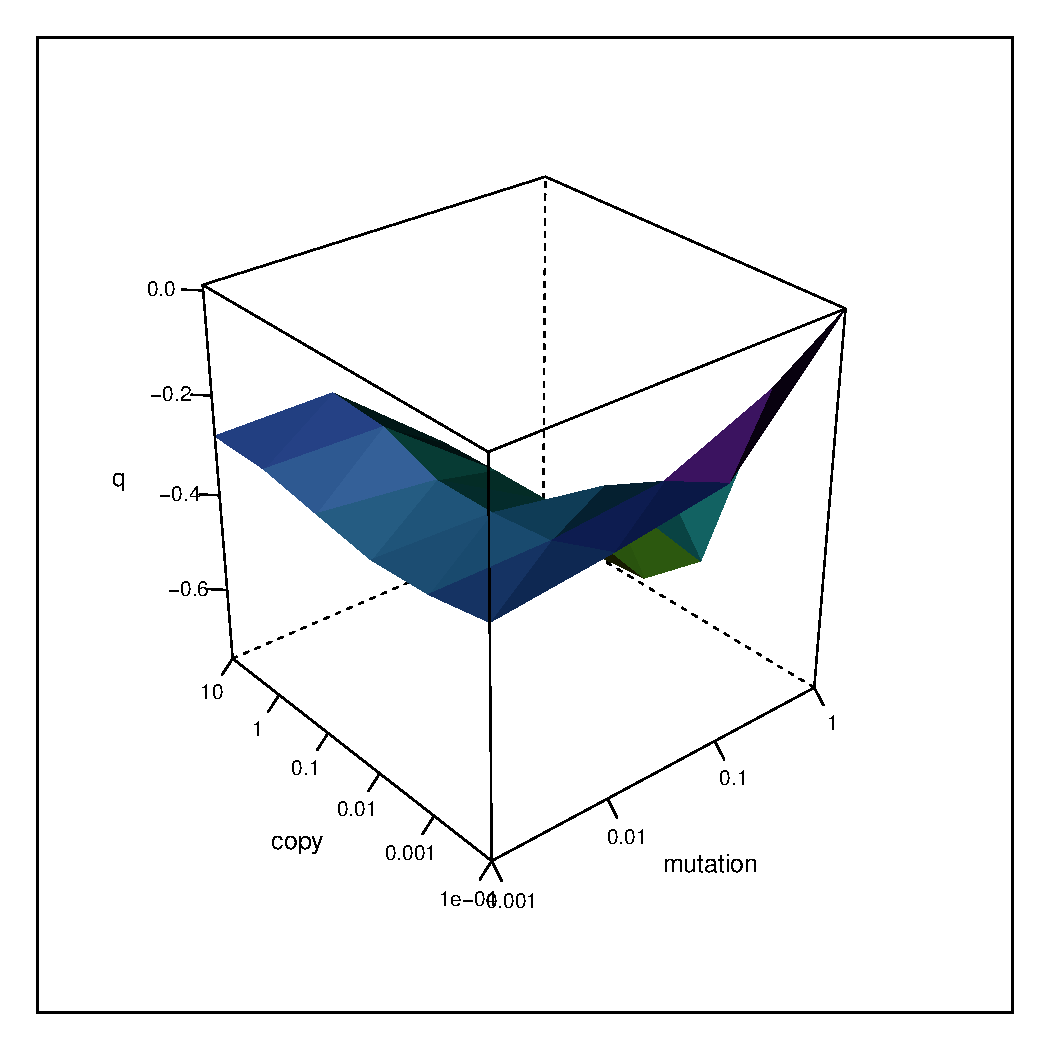
\includegraphics[height=2.5cm]{../images/QuantitieMuCopyAll.pdf}} &
	    \vspace{1cm}   \includegraphics[height=1.5cm]{../images/QuantitieCopyAll.pdf}&
	    \multirow{1}{2.5cm}{\includegraphics[height=2.5cm]{../images/PriceMuCopyAll.pdf}} &
	    \vspace{1cm} 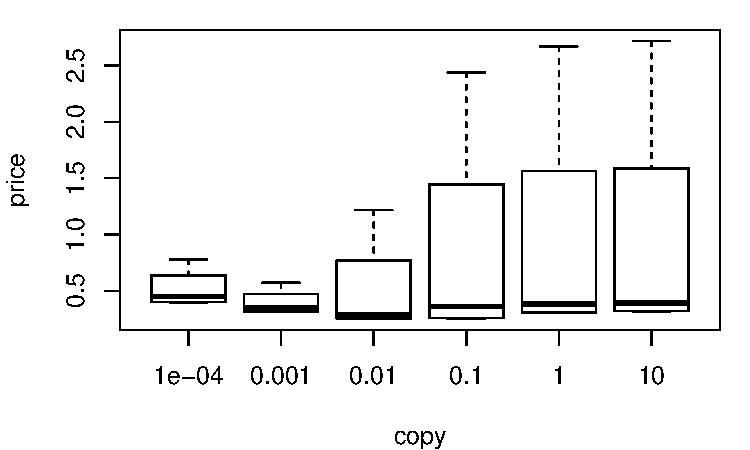
\includegraphics[height=1.5cm]{../images/PriceCopyAll.pdf} \\
	    &	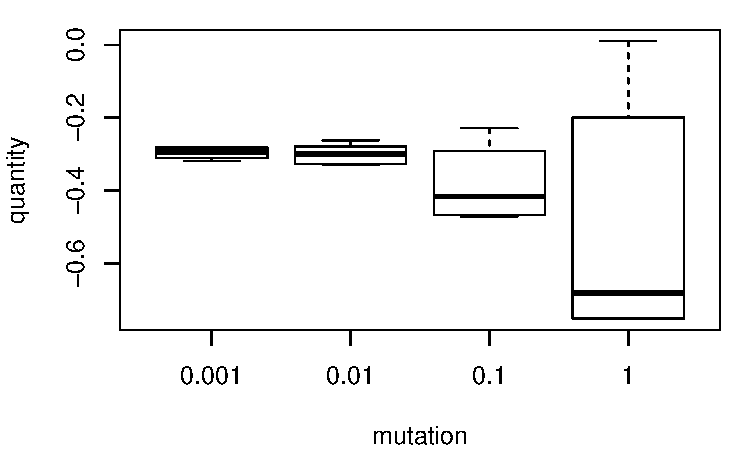
\includegraphics[height=1.5cm]{../images/QuantitieMuAll.pdf}&	&\includegraphics[height=1.5cm]{../images/PriceMuAll.pdf}\\
	\end{tabular}
    \end{table}
   
    \vspace{-1.5cm}

    \begin{table}

     \tiny Scores at the end
	\begin{tabular}{c m{2.5cm}}
	   \multirow{2}{2.5cm}{\includegraphics[height=2.5cm]{../images/ScoreMuCopyAll.pdf}} &
	   \vspace{1cm}\includegraphics[height=1.5cm]{../images/ScoreCopyAll.pdf}\\
	    & 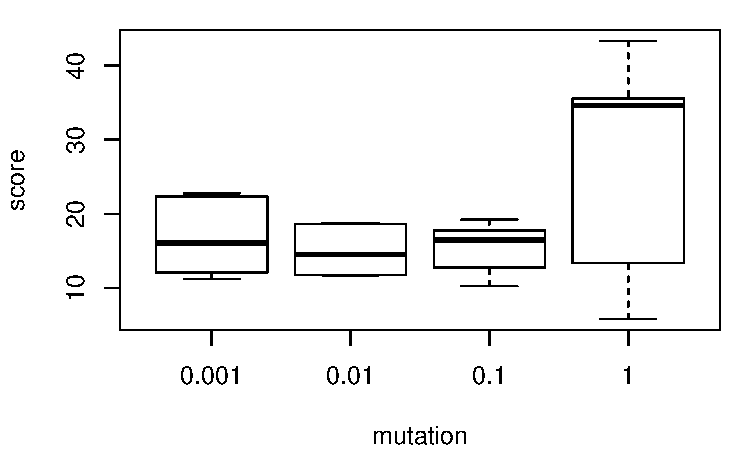
\includegraphics[height=1.5cm]{../images/ScoreMuAll.pdf} \\
	\end{tabular}
    \end{table}
\end{frame}

\begin{frame}{Chen et. Al 2017:The copy mechanism}
	\begin{columns}
		\begin{column}{.5\textwidth}
    \footnotesize
    A theoretical exploration of the model on Individual (Q-Learnign) vs social learning ($\lambda$).
		\end{column}
		\begin{column}{.5\textwidth}
    \begin{figure}
	
\includegraphics[width=\textwidth]{images/chenetAlComput.png}
    \end{figure}
		\end{column}
	\end{columns}
    \footnotesize
    \vspace{.5cm}


    %%\begin{table}
    %%\centering
    %% \tiny Prices at the end
    %%    \begin{tabular}{c m{2.5cm}}
    %%       \multirow{2}{2.5cm}{\includegraphics[height=2.5cm]{../images/PriceMuCopyAll.pdf}} &
    %%       \vspace{1cm}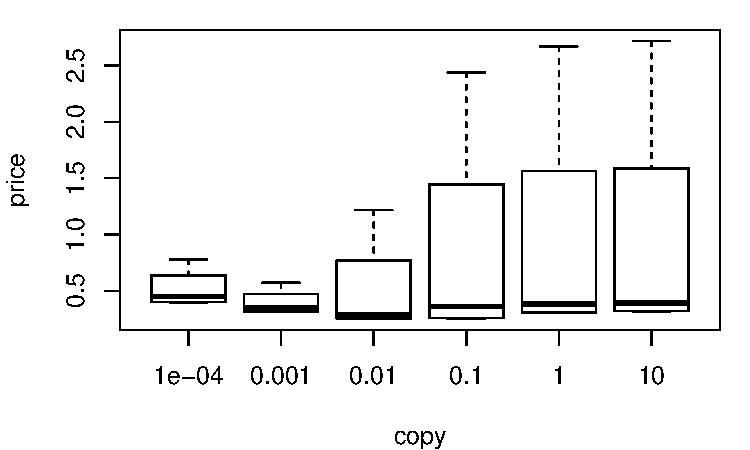
\includegraphics[height=1.5cm]{../images/PriceCopyAll.pdf}\\
    %%        & \includegraphics[height=1.5cm]{../images/PriceMuAll.pdf} \\
    %%    \end{tabular}
    %%\end{table}

    \textbf{ The ``intensity of choice'' ($\lambda$):}
    \begin{quote}
	\tiny
	 With higher $\lambda$'s, the agent’s choice is less random and is heavily
	 biased toward the better performing behavioral strategy; in other words, the degree of
	 exploration in which the agent engages is reduced. 
    \end{quote}
    \begin{figure}[htp]
	\begin{center}
	\begin{tabular}{m{4cm}cm{4cm}}
	   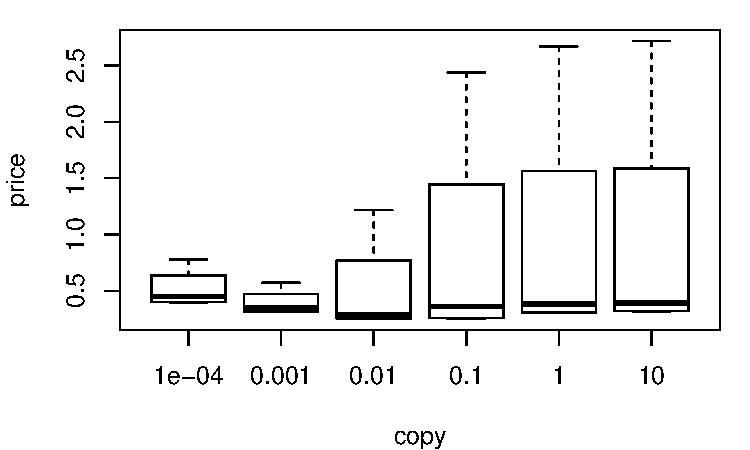
\includegraphics[height=2.5cm]{../images/PriceCopyAll.pdf} & vs  &
	     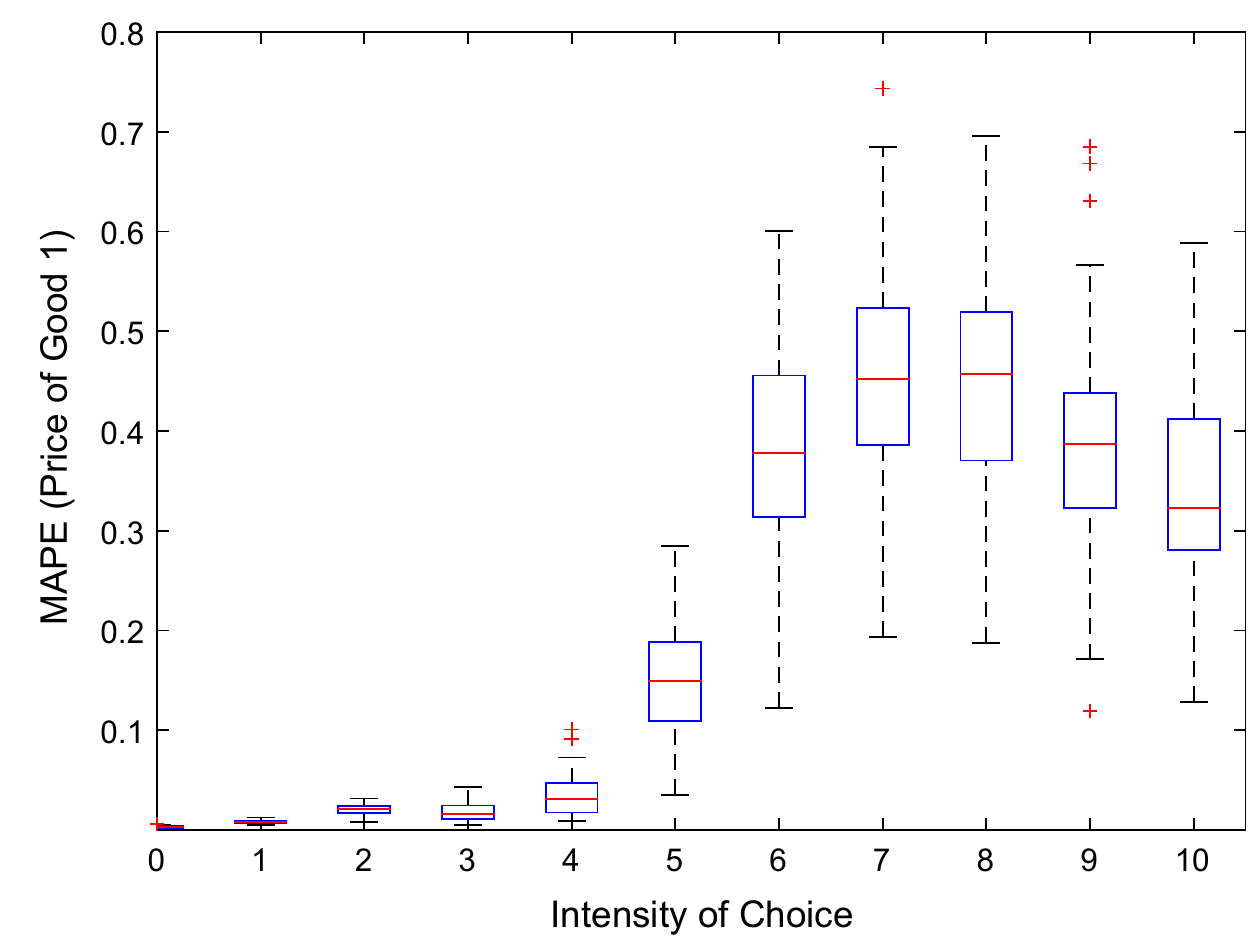
\includegraphics[height=2cm]{../images/chenetal_fig7.png} \\
	     \end{tabular}
	\end{center}
    \end{figure}
\end{frame}
\begin{frame}{Case study: Dynamics of changes}
    Final equilibrium state doesn't intereste us:\\

    {\centering $\rightarrow$ Dynamic of changes}

   
    \begin{itemize}
	\item Change in goods distribution
	\item Changes in sites diversity
    \end{itemize}
    
\end{frame}

\begin{frame}{Number of site with good 'N'}
    \small
Data \hfill Exp1 \hfill Exp2 \hfill Expe3 
	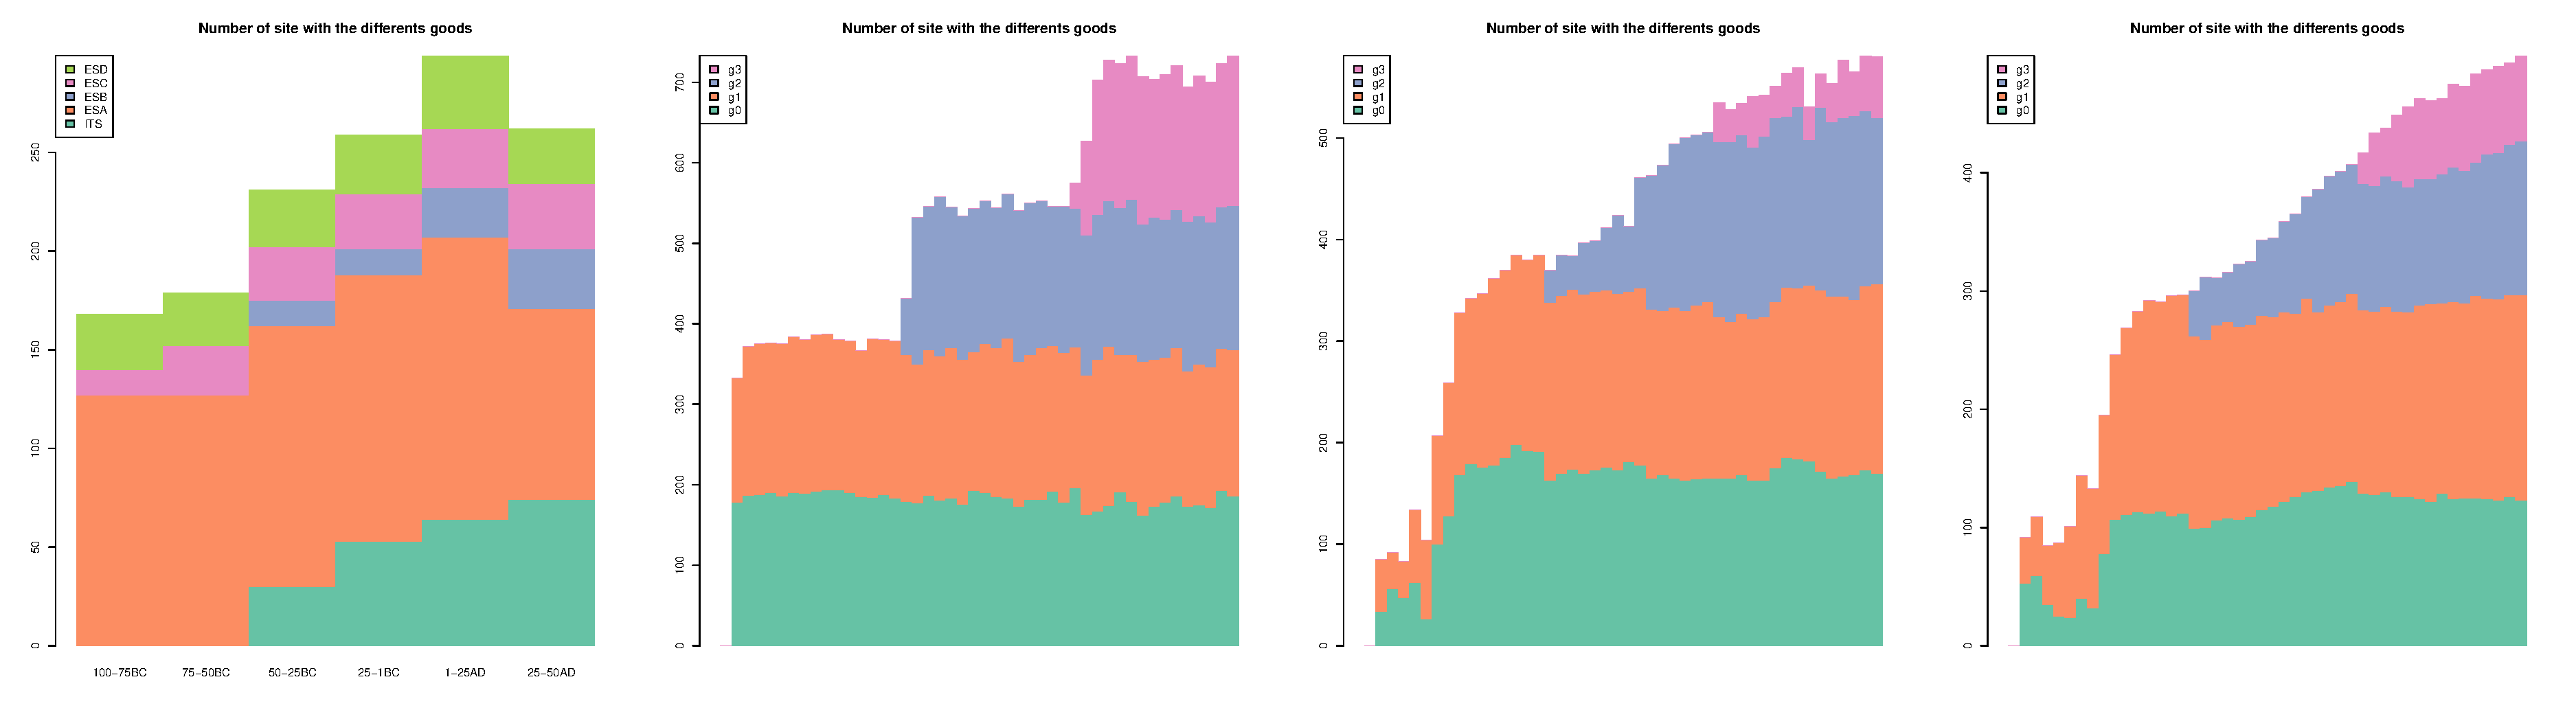
\includegraphics[width=\textwidth]{../images/hmNbSiteWGoodN.pdf}\\
	\includegraphics[width=\textwidth]{../images/plotNbSiteWGoodN.pdf}\\
\end{frame}

\begin{frame}{Number of site with 'N'differents goods}
    \centering
    \tiny
 Exp1 \hfill Exp2 \hfill Expe3 
	\includegraphics[width=.95\textwidth]{../images/hmNbGoodPerSite.pdf}\\
	\vfil
	\includegraphics[width=.95\textwidth]{../images/plotNbGoodPerSite.pdf}\\
\end{frame}


\begin{frame}{Impact of Social Learning }
 RDSendLine   The copy probability (\emph{ie} Chen's intensity of choice)
    $$\mu = 0.001$$
    $$\lambda  in \{0.0001,0.001,0.01,0.1,1,10\}$$
    \begin{center}
	\includegraphics[height=2cm]{{{../images/heatmap/heatMap-1_mu0.001-copy0.0001}}}
	\includegraphics[height=2cm]{{{../images/heatmap/heatMap-2_mu0.001-copy0.001}}}
	\includegraphics[height=2cm]{{{../images/heatmap/heatMap-3_mu0.001-copy0.01}}}
	\includegraphics[height=2cm]{{{../images/heatmap/heatMap-4_mu0.001-copy0.1}}}
	\includegraphics[height=2cm]{{{../images/heatmap/heatMap-5_mu0.001-copy1}}}
	\includegraphics[height=2cm]{{{../images/heatmap/heatMap-6_mu0.001-copy10}}}
    \end{center}

    \begin{center}
	\includegraphics[height=2cm]{{{../images/plot/plot-1_mu0.001-copy0.0001}}}
	\includegraphics[height=2cm]{{{../images/plot/plot-2_mu0.001-copy0.001}}}
	\includegraphics[height=2cm]{{{../images/plot/plot-3_mu0.001-copy0.01}}}
	\includegraphics[height=2cm]{{{../images/plot/plot-4_mu0.001-copy0.1}}}
	\includegraphics[height=2cm]{{{../images/plot/plot-5_mu0.001-copy1}}}
	\includegraphics[height=2cm]{{{../images/plot/plot-6_mu0.001-copy10}}}
    \end{center}
\end{frame}

\begin{frame}{Impact of Social Learning}
    The copy probability (\emph{ie} Chen's intensity of choice)
    $$\mu = 1$$
    $$\lambda \in \{0.0001,0.001,0.01,0.1,1,10\}$$
    \begin{center}
	\includegraphics[height=2cm]{{{../images/heatmap/heatMap-19_mu1-copy0.0001}}}
	\includegraphics[height=2cm]{{{../images/heatmap/heatMap-20_mu1-copy0.001}}}
	\includegraphics[height=2cm]{{{../images/heatmap/heatMap-21_mu1-copy0.01}}}
	\includegraphics[height=2cm]{{{../images/heatmap/heatMap-22_mu1-copy0.1}}}
	\includegraphics[height=2cm]{{{../images/heatmap/heatMap-23_mu1-copy1}}}
	\includegraphics[height=2cm]{{{../images/heatmap/heatMap-24_mu1-copy10}}}
    \end{center}

    \begin{center}
	\includegraphics[height=2cm]{{{../images/plot/plot-19_mu1-copy0.0001}}}
	\includegraphics[height=2cm]{{{../images/plot/plot-20_mu1-copy0.001}}}
	\includegraphics[height=2cm]{{{../images/plot/plot-21_mu1-copy0.01}}}
	\includegraphics[height=2cm]{{{../images/plot/plot-22_mu1-copy0.1}}}
	\includegraphics[height=2cm]{{{../images/plot/plot-23_mu1-copy1}}}
	\includegraphics[height=2cm]{{{../images/plot/plot-24_mu1-copy10}}}
    \end{center}
\end{frame}

\begin{frame}{Impact innovation rate}
    The mutation rate (\emph{ie} internal innovation rate, random change of a price)
    $$\mu \in \{0.001,0.01,0.1,1\}$$
    $$\lambda = 0.0001$$
    \begin{center}
	\includegraphics[height=2cm]{{{../images/heatmap/heatMap-1_mu0.001-copy0.0001}}}
	\includegraphics[height=2cm]{{{../images/heatmap/heatMap-7_mu0.01-copy0.0001}}}
	\includegraphics[height=2cm]{{{../images/heatmap/heatMap-13_mu0.1-copy0.0001}}}
	\includegraphics[height=2cm]{{{../images/heatmap/heatMap-19_mu1-copy0.0001}}}
    \end{center}

    \begin{center}
	\includegraphics[height=2cm]{{{../images/plot/plot-1_mu0.001-copy0.0001}}}
	\includegraphics[height=2cm]{{{../images/plot/plot-7_mu0.01-copy0.0001}}}
	\includegraphics[height=2cm]{{{../images/plot/plot-13_mu0.1-copy0.0001}}}
	\includegraphics[height=2cm]{{{../images/plot/plot-19_mu1-copy0.0001}}}
    \end{center}
\end{frame}

\begin{frame}{Impact innovation rate}
    The mutation rate (\emph{ie} internal innovation rate, random change of a price)
    $$\mu \in \{0.001,0.01,0.1,1\}$$
    $$\lambda = 10$$
    \begin{center}
	\includegraphics[height=2cm]{{{../images/heatmap/heatMap-6_mu0.001-copy10}}}
	\includegraphics[height=2cm]{{{../images/heatmap/heatMap-12_mu0.01-copy10}}}
	\includegraphics[height=2cm]{{{../images/heatmap/heatMap-18_mu0.1-copy10}}}
	\includegraphics[height=2cm]{{{../images/heatmap/heatMap-24_mu1-copy10}}}
    \end{center}

    \begin{center}
	\includegraphics[height=2cm]{{{../images/plot/plot-6_mu0.001-copy10}}}
	\includegraphics[height=2cm]{{{../images/plot/plot-12_mu0.01-copy10}}}
	\includegraphics[height=2cm]{{{../images/plot/plot-18_mu0.1-copy10}}}
	\includegraphics[height=2cm]{{{../images/plot/plot-24_mu1-copy10}}}
    \end{center}

\end{frame}

\begin{frame}{Hidden changes}
	Means of non normal distributions!

	change of the whole \emph{distribution}  of how the simulations end, not just moving the mean 
	\begin{center}
	    $\rightarrow$ Some parameters lead to totally differents simulations, other no
	\end{center}
	

    \end{frame}

\begin{frame}{Distribution of simulations output}
    \tiny

	\begin{table}
	    \begin{tabular}{m{2.1cm}m{2.1cm}m{2.1cm}m{2.1cm}}
		expe & general & distrib $1Goods$ & distrib $5Goods$ \\
		mu0.001-copy0.0001 & 

		\includegraphics[height=2cm]{{{../images/plot/plot-1_mu0.001-copy0.0001}}} &
		\includegraphics[height=2cm]{{{../images/distrib-1goods-9000timstep-exp1_mu0.001-copy0.0001}}} &
		\includegraphics[height=2cm]{{{../images/distrib-5goods-9000timstep-exp1_mu0.001-copy0.0001}}} \\

		mu0.01-copy0.0001 & 

		\includegraphics[height=2cm]{{{../images/plot/plot-7_mu0.01-copy0.0001}}} &
		\includegraphics[height=2cm]{{{../images/distrib-1goods-9000timstep-exp7_mu0.01-copy0.0001}}} &
		\includegraphics[height=2cm]{{{../images/distrib-5goods-9000timstep-exp7_mu0.01-copy0.0001}}} \\


		mu0.001-copy10 & 

		\includegraphics[height=2cm]{{{../images/plot/plot-6_mu0.001-copy10}}} &
		\includegraphics[height=2cm]{{{../images/distrib-1goods-9000timstep-exp6_mu0.001-copy10}}} &
		\includegraphics[height=2cm]{{{../images/distrib-5goods-9000timstep-exp6_mu0.001-copy10}}} \\

		mu0.01-copy10 & 

		\includegraphics[height=2cm]{{{../images/plot/plot-12_mu0.01-copy10}}} &
		\includegraphics[height=2cm]{{{../images/distrib-1goods-9000timstep-exp12_mu0.01-copy10}}} &
		\includegraphics[height=2cm]{{{../images/distrib-5goods-9000timstep-exp12_mu0.01-copy10}}} \\

	    \end{tabular}
	\end{table}

\end{frame}

\begin{frame}{Approximate Bayesian Computation}
    We can compute for each simulation of a given set of parameter the distance to the data.
    Thus we can know for which value of paramaters our model is the more probable to reproduce the real data.
\end{frame}

\begin{frame}{Trieste Case Study}
    \begin{itemize}
	\item $\approx 200$ goods from steal and grain, to wooden clock and card games.
	\item Going to and from $\approx 400$ different ports
	\item 60 years
    \end{itemize}
    \begin{figure}[h]
	\includegraphics[width=.45\textwidth]{images/distribgood66.pdf}
	\includegraphics[width=.45\textwidth]{images/distribgood76.pdf}
    \end{figure}
\end{frame}

\begin{frame}{Trieste Case Study}
    \begin{itemize}
	\item Does a simple decentralized model of economy reproduce some of the observed patterns?
	\item How the paramters differents from previous cas study (\emph{ie} highe $\lambda$: role of exchange more important, greater $\mu$, higher rates of innovations\dots
    \end{itemize}
\end{frame}

\begin{frame}
	\begin{center}
		\Large
		or not.
		%Thank for you attention!\\
%		What was the nature of Roman economy?\\
%		\includegraphics[width=2cm]{images/LOGO-ERC.jpg} \hfil	\includegraphics[width=3cm]{../../logos/epnetLogo.png}\\
%		\vspace{1cm}
%		\scriptsize
%			http://www.roman-ep.net/\\
%			@epnetproject\\
%			fb.com/EPNetProject\\
%			@simoncarrignon
	\end{center}


\end{frame}

%\begin{frame}
%    \Huge
%    Thank for you attention!
%\end{frame}
\end{document}


